\label{sec:session}
\chapter{Algorithm Implementation}

\section{Clustering Techniques}

K-means Implementation: Explanation of parameter tuning (e.g., choosing the optimal number of clusters using the Elbow Method or Silhouette Score).

DBSCAN Implementation: Explanation of key parameters (eps, min\_samples) and how they were optimized.

Gaussian Mixture Models (GMM): Justification for using GMM and how covariance structures were selected.

Hierarchical Clustering (if used): Description of dendrogram-based analysis and how clusters were formed.

Python Code Snippets: Example implementations of each method.

\section{Dimensionality Reduction}

PCA Implementation: Details on how many components were retained and why.

Explained Variance Ratio: Table showing variance retained per principal component.

Python Code Snippets: Code to execute PCA.

\section{Regime-Switching Models}

Markov-Switching GARCH (MS-GARCH): Explanation of model selection, estimated parameters, and validation.

Python Code Snippets: MS-GARCH implementation using statsmodels.

%% This shows appendix shows how to attach a file to the appendix.
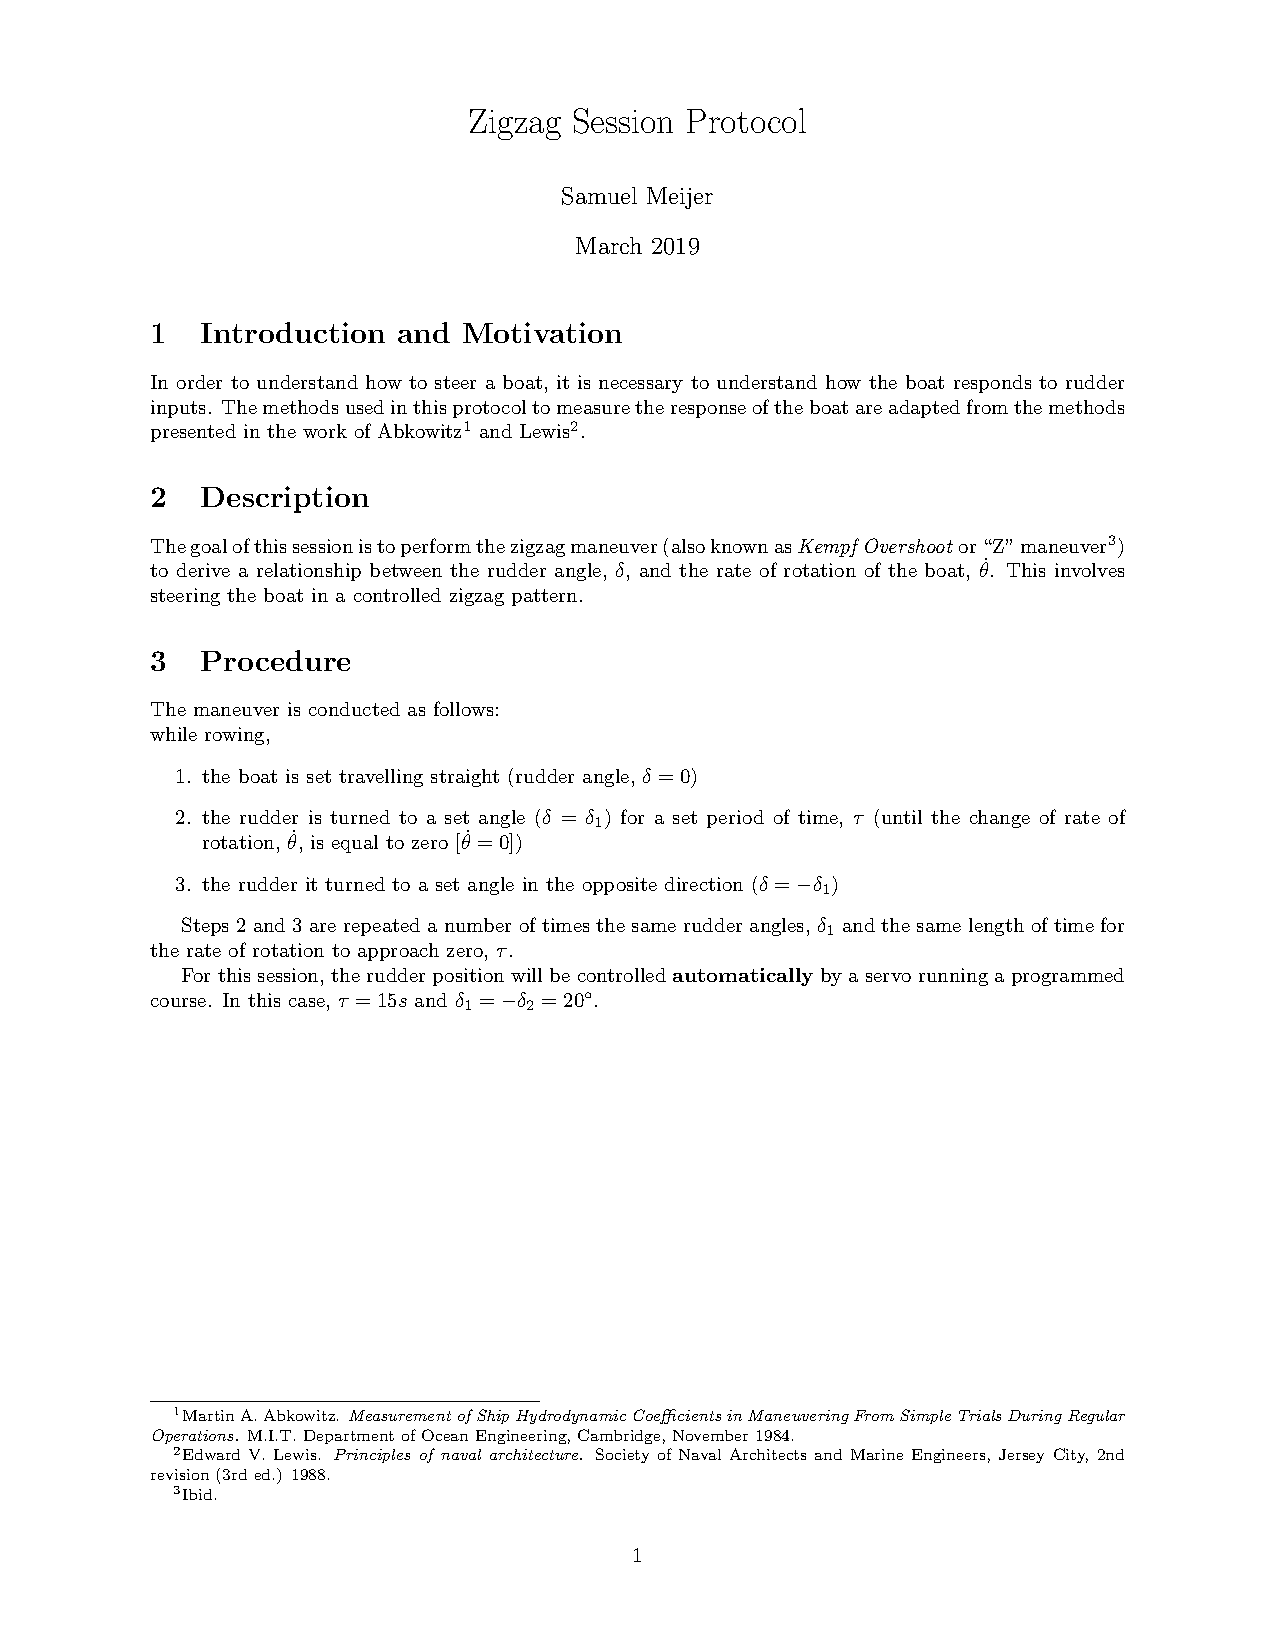
\includepdf[]{appendices/Session_Protocol-3.pdf}
